\newcommand{\labtitle}{ECE/CS 5710/6710 - Lab 3}
\newcommand{\labsubtitle}{Synthesis of a MIPS Processor}
\vlsiheader

\begin{center}
\LARGE\textbf{\labsubtitle} \\
	\large\textbf{Pre-lab Assignment:} Check for the date on Canvas. \\
	\large\textbf{Lab Report:} Check for the date on Canvas.
\end{center}
\section{Objective}
This lab presents the main steps for performing the RTL/logic synthesis of an 8-bit MIPS microprocessor from the \textit{CMOS VLSI Design} book, using the Skywater 130 \emph{nm} design kit. This lab details the typical steps of the logic synthesis in VLSI design. The tool you will use is Synopsys Design Compiler\textsuperscript{\tiny\textregistered}, which is widely used in industry and academia. 



\section{Pre-lab Assignment}
\begin{prelab}
	Answer the following questions and submit a \textbf{.pdf} file through Canvas:
 \begin{enumerate}
 	\item What RTL stands for? Explain briefly the different levels of abstraction in VLSI design.
 	\item Explain briefly what is logic synthesis in VLSI design.
 	\item What is a timing library and what does it contain? Why do you need it for the synthesis flow?
 \end{enumerate}
\vspace{-5mm}
\end{prelab}


\section{Directory Organization}

For the logic synthesis, it will be simplest to work from a \textit{design$\_$compiler} folder. This folder has been added to the git repo. If it does not exist, the repo can be updated with:

\begin{codeline}
	git pull
\end{codeline}

This folder contains different subdirectories as follows:
 \begin{itemize}
\item \textit{DDC}: design database, where you will save your design after the different steps of the synthesis.
\item \textit{RPT}: report files (area, gate etc.) created by the tool.
\item \textit{SDC}: system design constraint file created by the tool.
\item \textit{SCRIPTS}: contains a TCL script to automatize the synthesis step (to be used at the end of the lab).
\item \textit{SDF}: Timing files created by the tool for functional verification.
\end{itemize}





\section{Lab Assignment}


\subsection{Starting Synopsys Design Compiler\textsuperscript{\tiny\textregistered}}
Launch the Synopsys Design Compiler\textsuperscript{\tiny\textregistered} GUI by going in your \textit{design$\_$compiler} folder and doing:
	\begin{codeline}
	design$\_$vision
\end{codeline}

The \textit{design$\_$compiler} directory contains an hidden file named \textit{.synopsys$\_$dc.setup}. This file is read every time Synopsys DC starts.
It specify what is the target library (the library that defines the area/timing/power characteristics of the physical logic gates) so in our case the standard cells from Skywater 130 \emph{nm}).\\


When Synopsys DC is opened, you will obtain a window as shown in Fig \ref{fig_syn_dc}. The \textbf{\textcolor{blue}{Console terminal}} is used for entering Design Compiler (DC) commands, to source Tcl scripts or to run Linux commands. Those things can also be done through the \textbf{\textcolor{blue}{command line}} through a script. The lab will show you how to perform the tasks with the GUI by hand, but it can be automatized by running command lines. In addition, not all commands are available in the GUI. For more complex and repetitive synthesis tasks, it is highly recommended to use scripts. When you will perform actions on the GUI, the equivalent commands will be recorded and stored in the \textit{command.log} file in the \textit{design$\_$compiler} directory. The equivalent commands will also be given in this tutorial. To obtain some help about a command, you can run in the console terminal or the command line: 	

	\begin{codeline}
	man your$\_$command
\end{codeline}


\begin{figure}[!h]
	\centering
	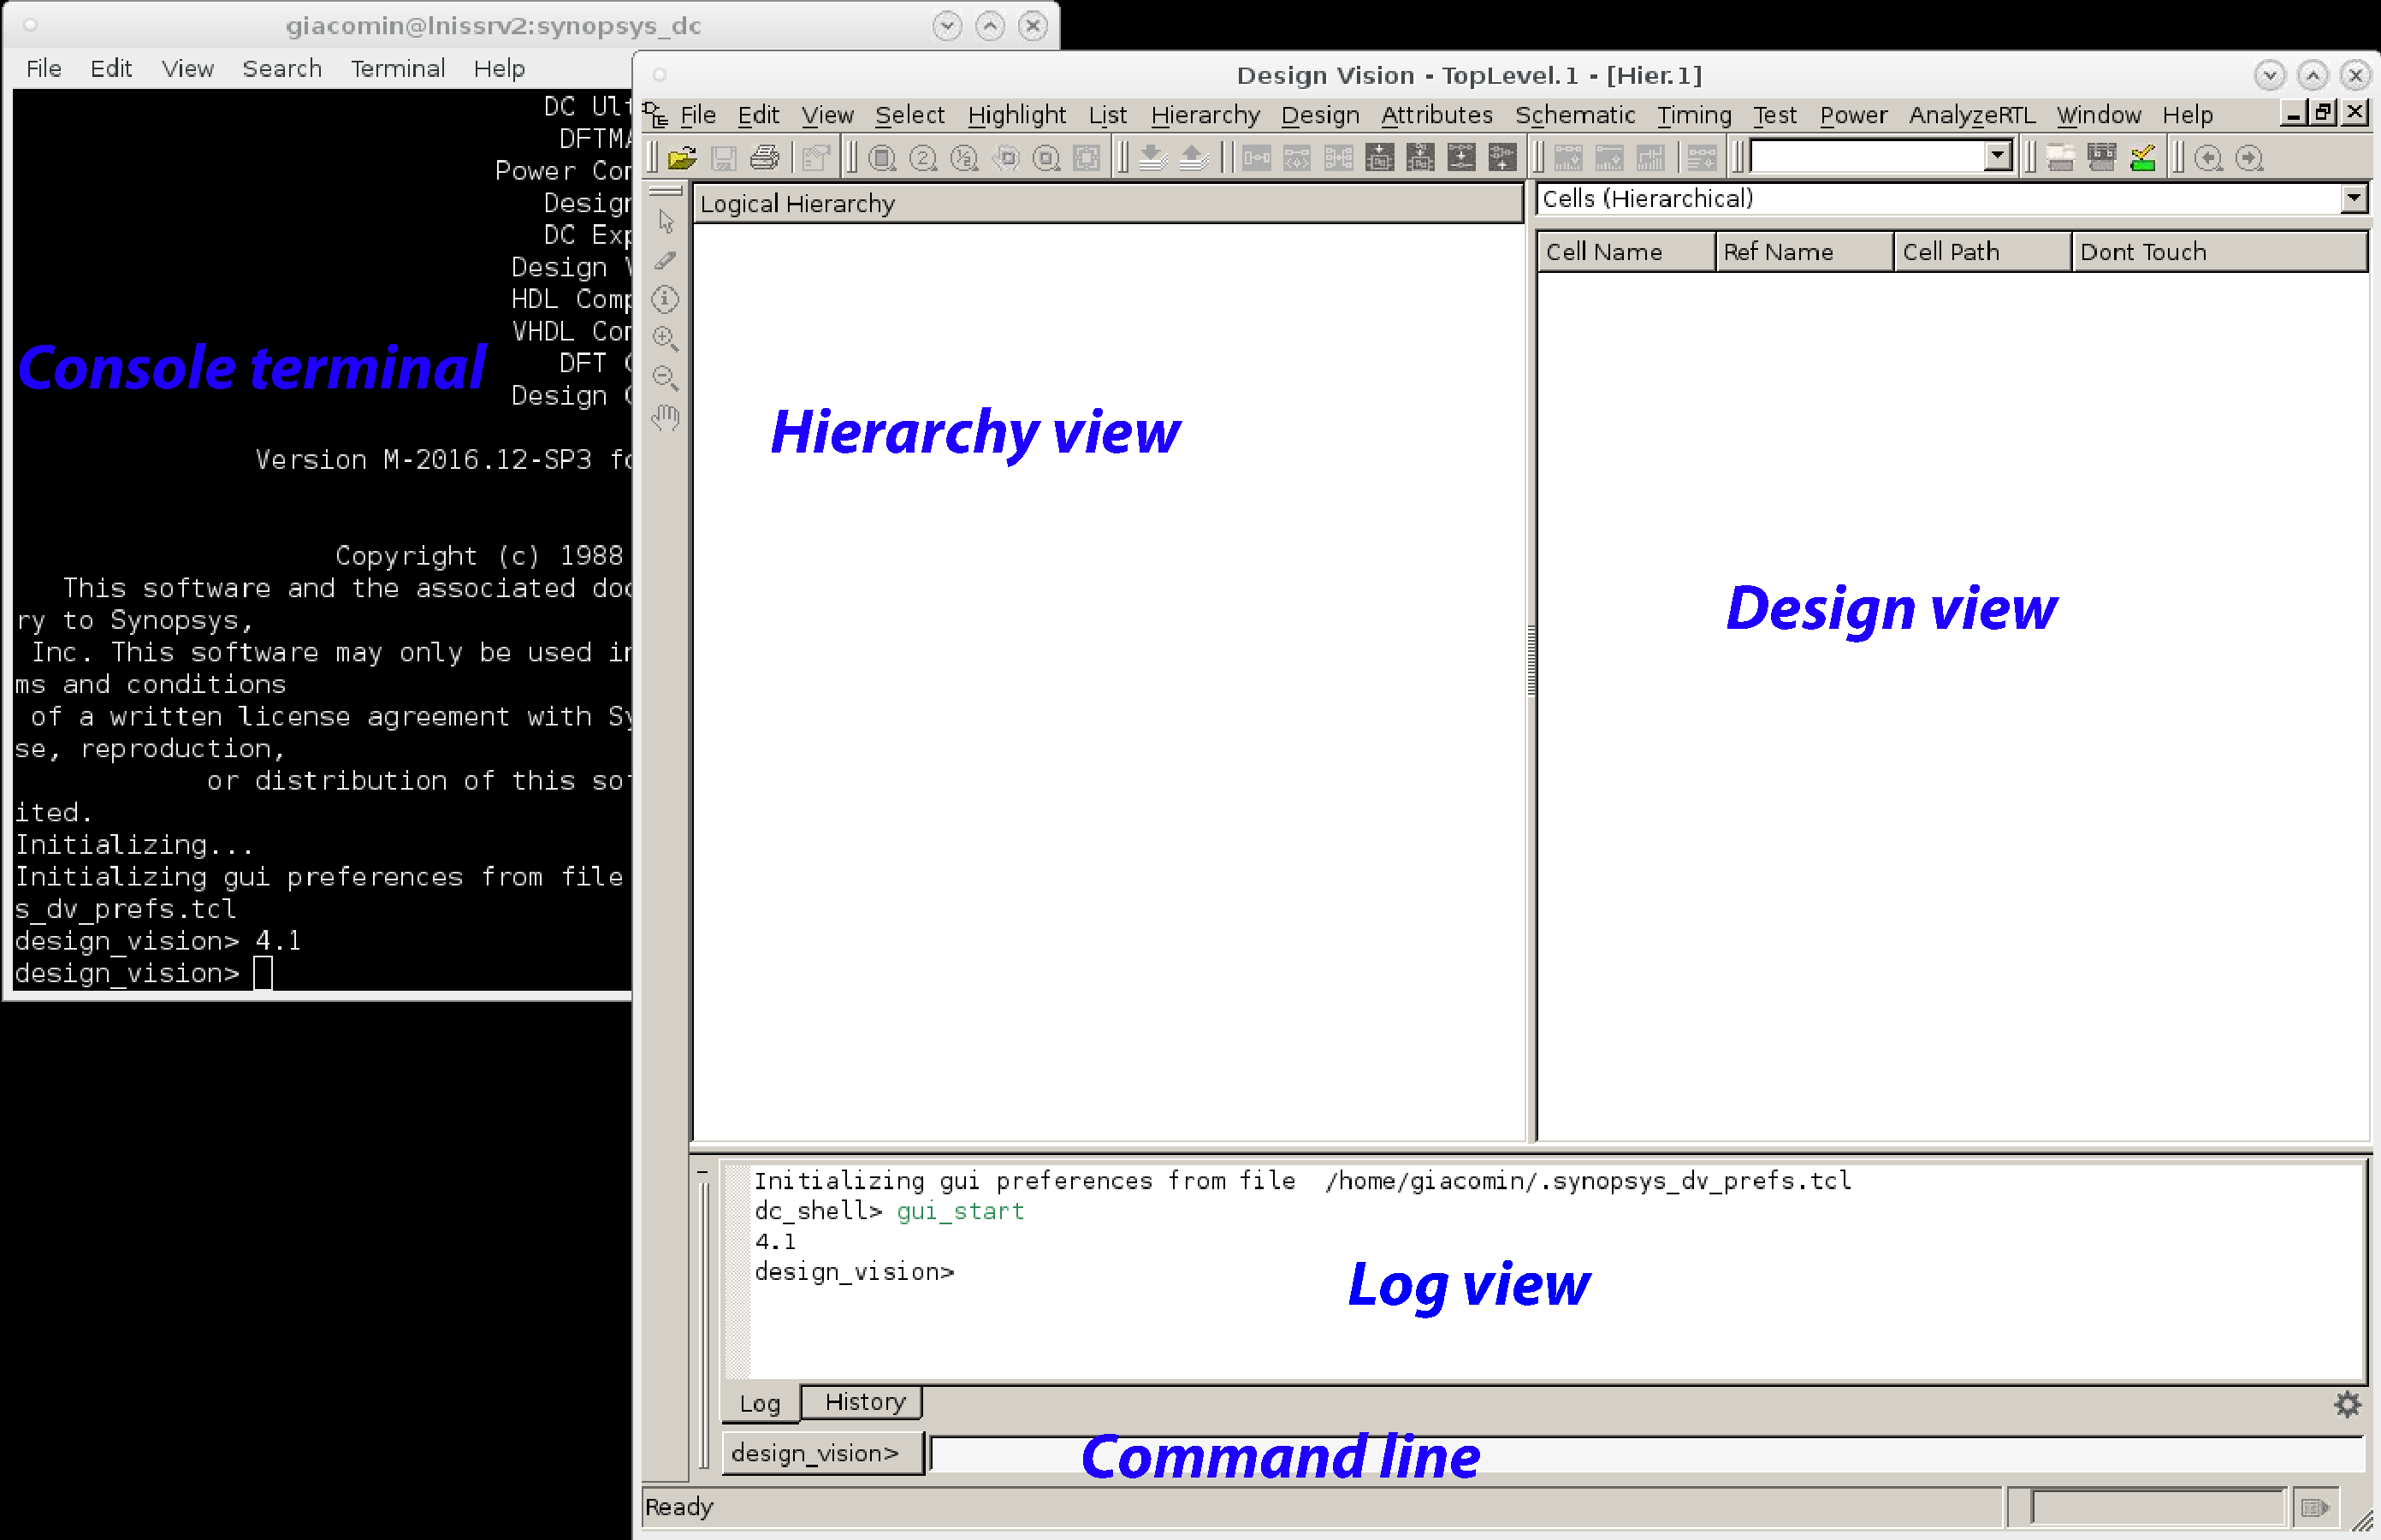
\includegraphics[scale=0.33]{figures/lab3_design_compiler/synopsys_overall.pdf}
	\caption{Synopsys DC window organization}
	\label{fig_syn_dc}
\end{figure}



The console terminal and the \textit{Log} view contain the trace of the execution of the command. The \textit{History} tab contains the history of all executed commands in the session.

\subsection{Analyzing the Verilog RTL Files}

	\parbox[t]{\dimexpr\textwidth-\leftmargin}{%
	\begin{wrapfigure}[11]{r}{0.4\textwidth}
		\vspace{-6mm}
		\centering
		\vspace{-\baselineskip}
 		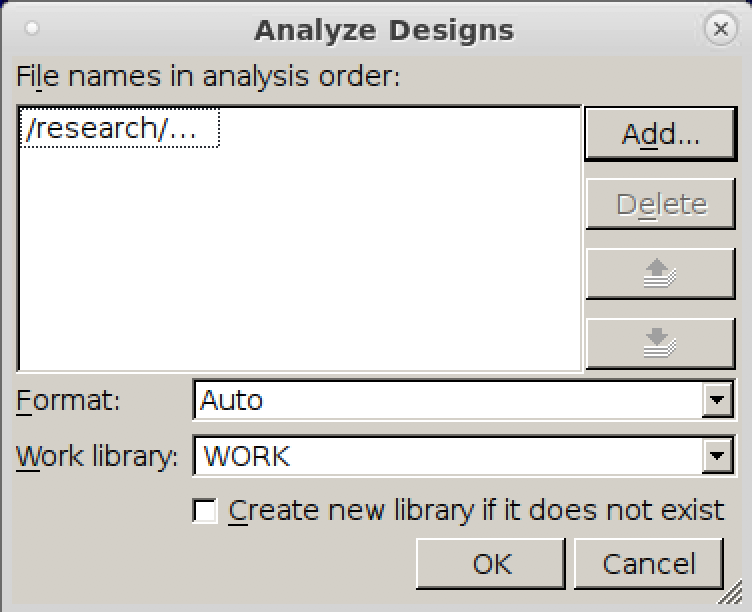
\includegraphics[scale=0.5]{figures/lab3_design_compiler/analyze_dc}
\caption{Analyzing the Design}
\label{fig_analyze_dc}
	\end{wrapfigure}
	The analysis phase will compile the Verilog or VHDL source files and ensure that they are synthesizable (that means that they only contains statement that have meaning for synthesis, i.e. that can be mapped into a hardware circuit). To analyze the files, do:
	 \begin{enumerate}
		\item \textit {File -> Analyze...}
		\item Click on the \textit{Add...} button, as shown in Fig \ref{fig_analyze_dc} to select the Verilog file of the 8-bit microprocessor (\textit{mips.sv}). It is located in the \textit{HDL/RTL} folder.
		\item Click on OK.	
	\end{enumerate}
}

Equivalent DC command:
	\begin{codeline}
	analyze -library WORK -format sverilog $\{$.../HDL/RTL/mips.v$\}$
\end{codeline}

\subsection{Elaborating the Design}

	\parbox[t]{\dimexpr\textwidth-\leftmargin}{%
	\begin{wrapfigure}[11]{r}{0.4\textwidth}
		\vspace{-6mm}
		\centering
		\vspace{-\baselineskip}
		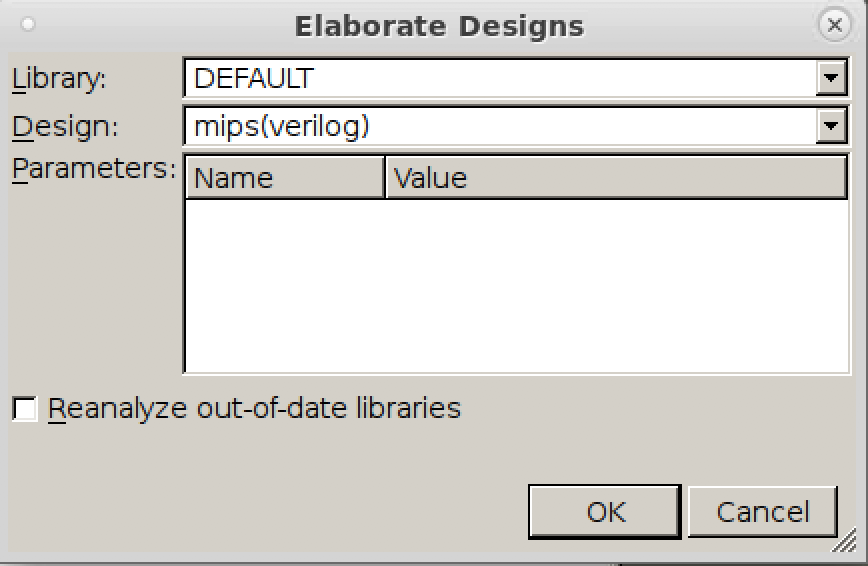
\includegraphics[scale=0.45]{figures/lab3_design_compiler/elaborate_dc}
\caption{Elaborating the design}
\label{fig_elaborate_dc}
	\end{wrapfigure}
This phase will perform a pre-synthesis of the netlist. It will basically identify the logic functions and the different registers (latches and flip-flops) that will be inferred. To elaborate the design, do:

\begin{enumerate}
	\item \textit {File -> Elaborate...}
	\item Select the top module of the verilog netlist: \textit{Processor}, as shown in Fig \ref{fig_analyze_dc}. 
	\item Click on OK.	
\end{enumerate}
}




Equivalent DC command:
	\begin{codeline}
elaborate mips -architecture verilog -library DEFAULT
\end{codeline}


On the \textbf{\textcolor{blue}{Log window}}, you can see the inferred registers for the different modules, as shown in Fig \ref{fig_registers}, their size (width) and their Set/Reset signals (AR/AS: asynchronous reset/set, SR/SS: synchronous reset/set). 

	\begin{figure}[!h]
	\centering
	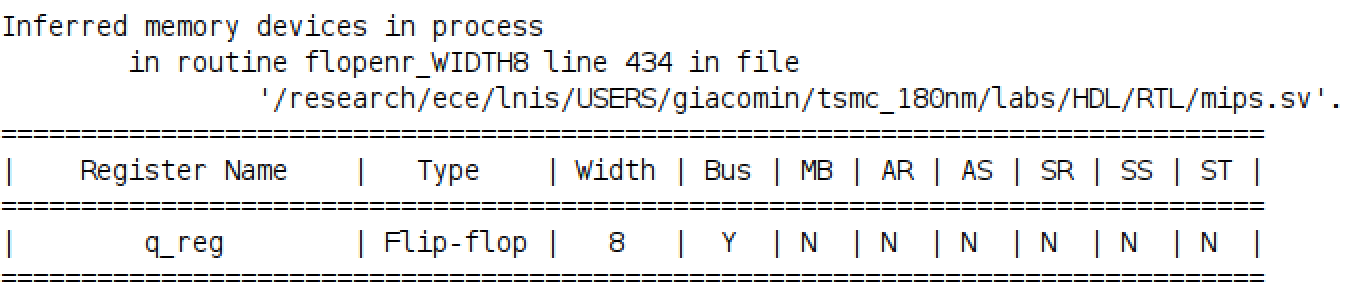
\includegraphics[scale=0.5]{figures/lab3_design_compiler/registers}
	\caption{Some of the inferred registers}
	\label{fig_registers}
\end{figure}

On the \textbf{\textcolor{blue}{Hierarchy view}}, you can now see the inferred components and the associated standard logic cells. Select the \textit{andblock} from the \textit{alunit} module, as shown in Fig. \ref{fig_cellall} and select \textit{Cells (All)} at the top of the design view. It is also possible to display the elaborated schematics. Lets do it for the \textit{andblock}. To do so, make sure that the \textit{andblock} instance is selected in the hierarchy view and click on the \textit{Create Design Schematic} icon, as depicted in Fig. \ref{fig_cellall}. A new window containing the \textit{andblock} schematic now opens.

	\begin{figure}[!h]
	\centering
	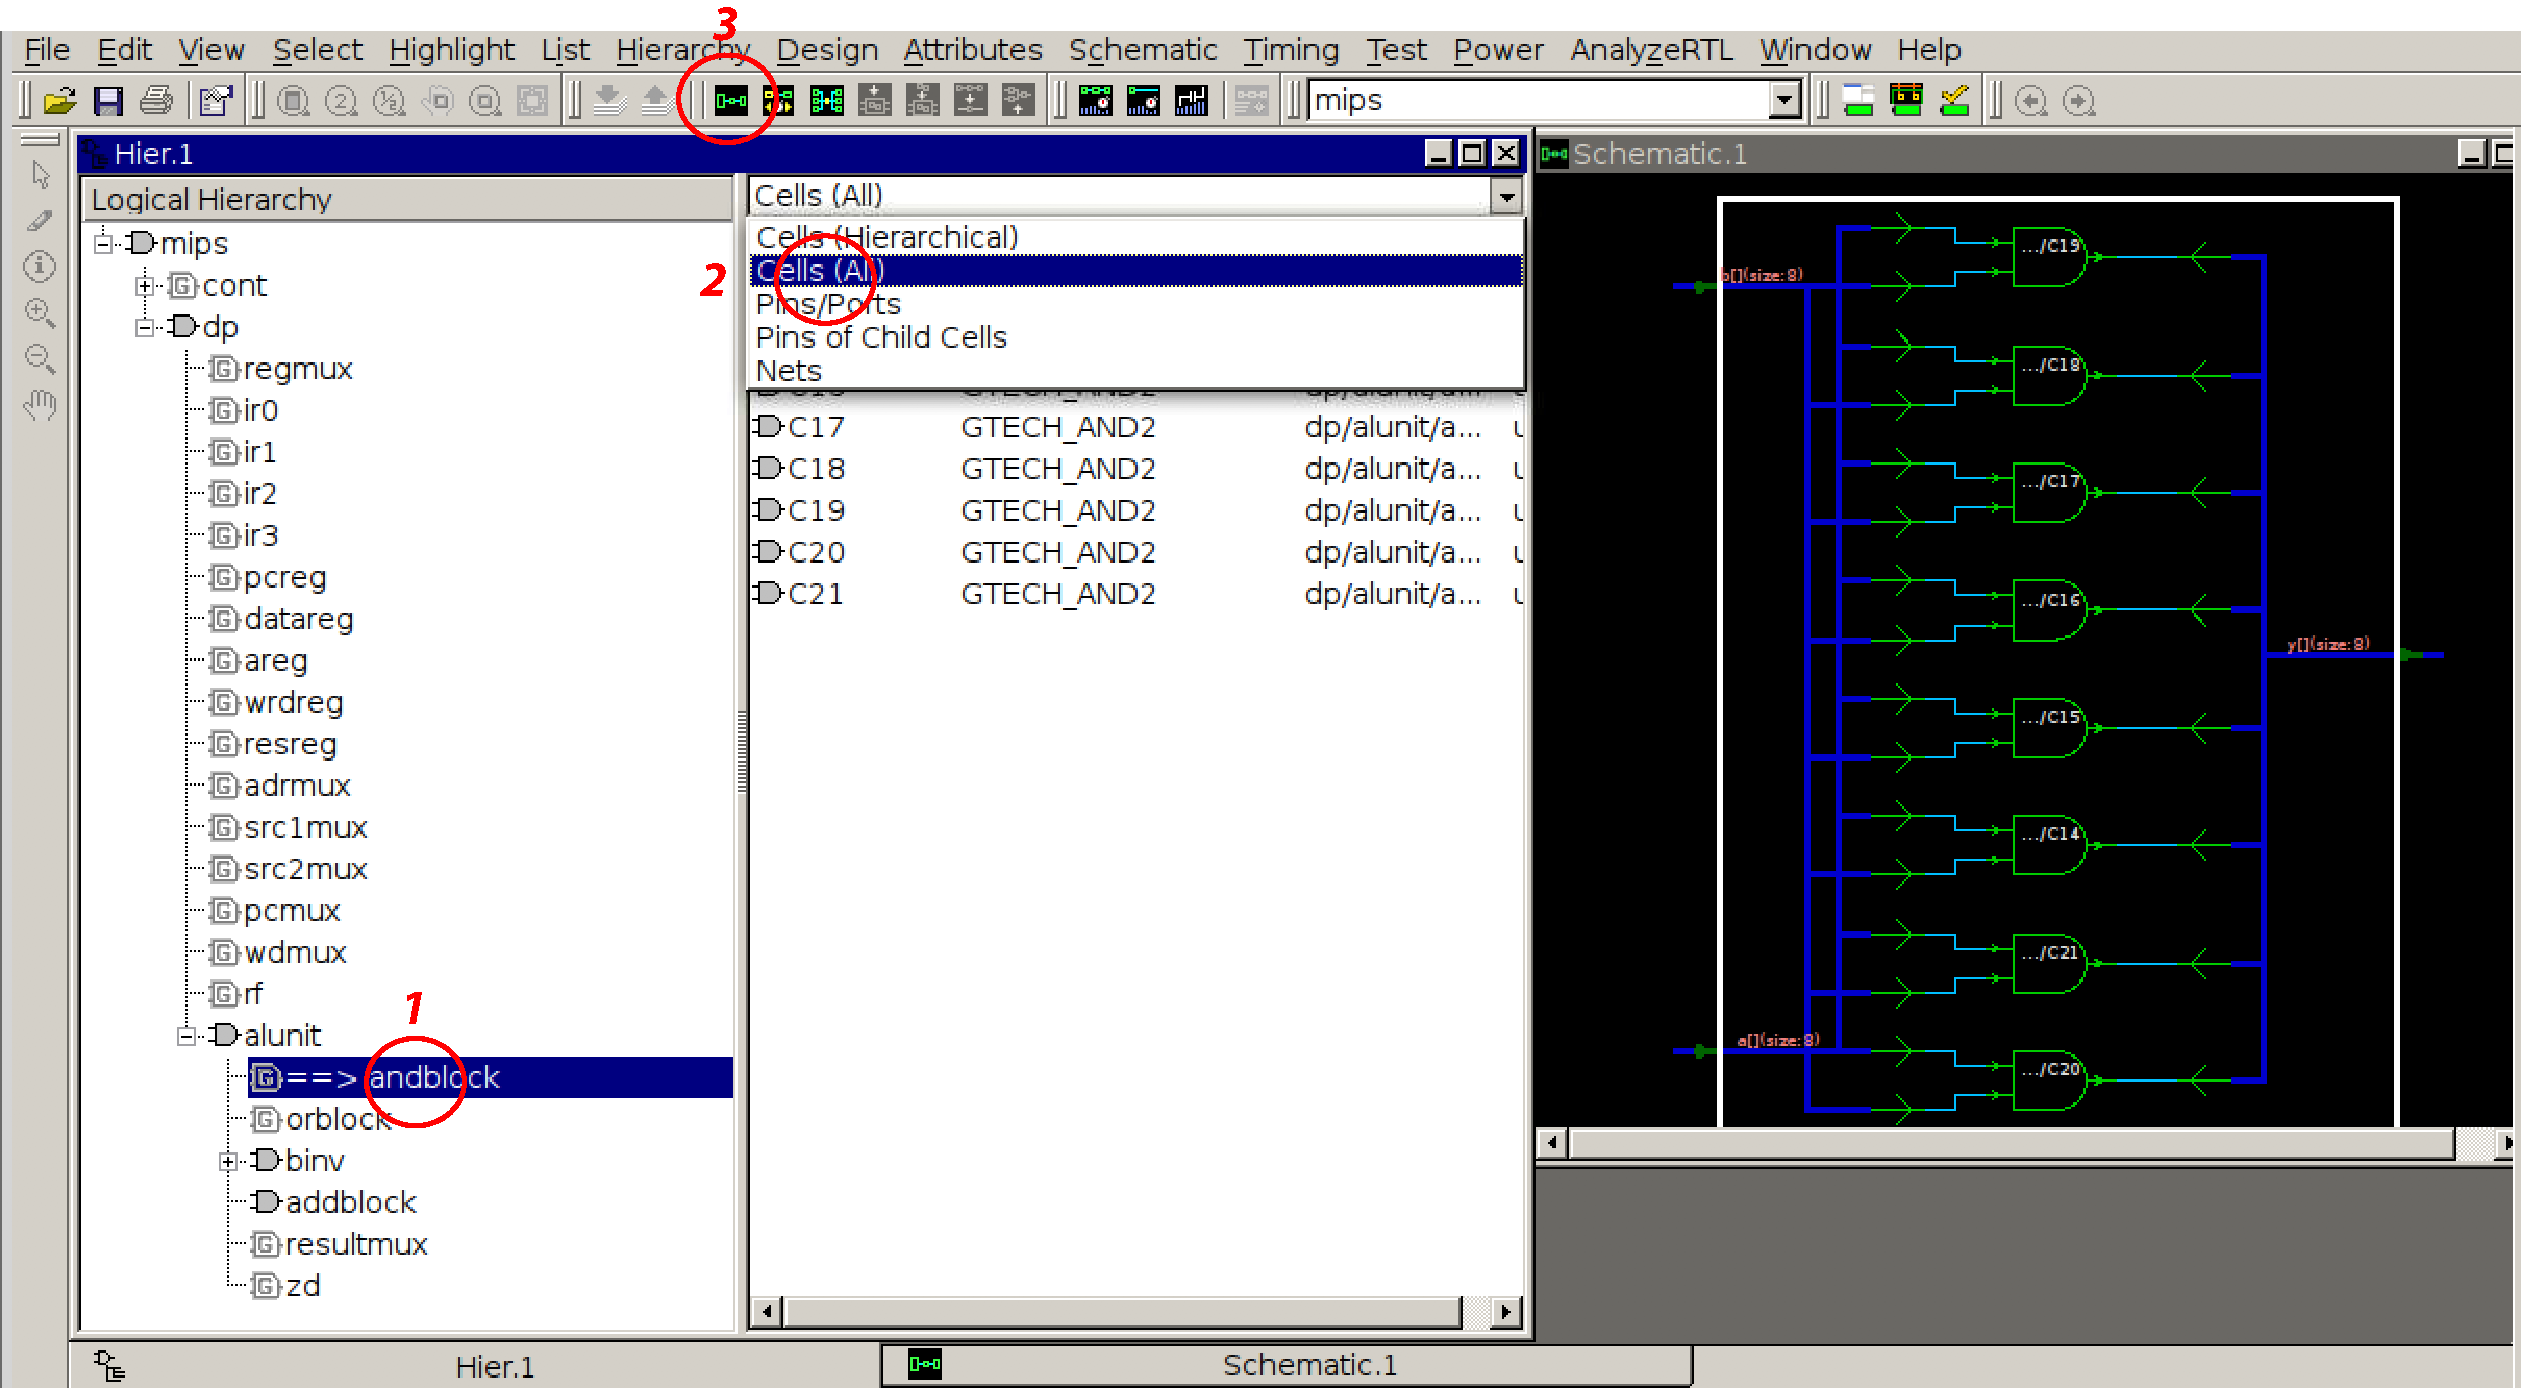
\includegraphics[scale=0.32]{figures/lab3_design_compiler/cellall.pdf}
	\caption{Displaying all cells and creating the schematic of the 8-bit AND.}
	\label{fig_cellall}
\end{figure}
		\vspace{-6mm}
\begin{remark}
 The GTECH$\_$XXX elements are denoting generic combinational logic functions which are not mapped to the standard cell library yet. In other modules, you can find names starting with a * (e.g.*ADD, *SUB etc.) which denote more complex generic combinational operators. The reference name **logic0** or **logic1** denotes a wire tied to 0 ($G_{ND}$) or tied to 1 ($V_{DD}$), respectively and the reference name **SEQGEN** denotes a flip-flop register.
 \end{remark}
 
\subsection{Saving and Restoring the Design}
	\parbox[t]{\dimexpr\textwidth-\leftmargin}{%
	\begin{wrapfigure}[11]{r}{0.4\textwidth}
		\vspace{-6mm}
		\centering
		\vspace{-\baselineskip}
		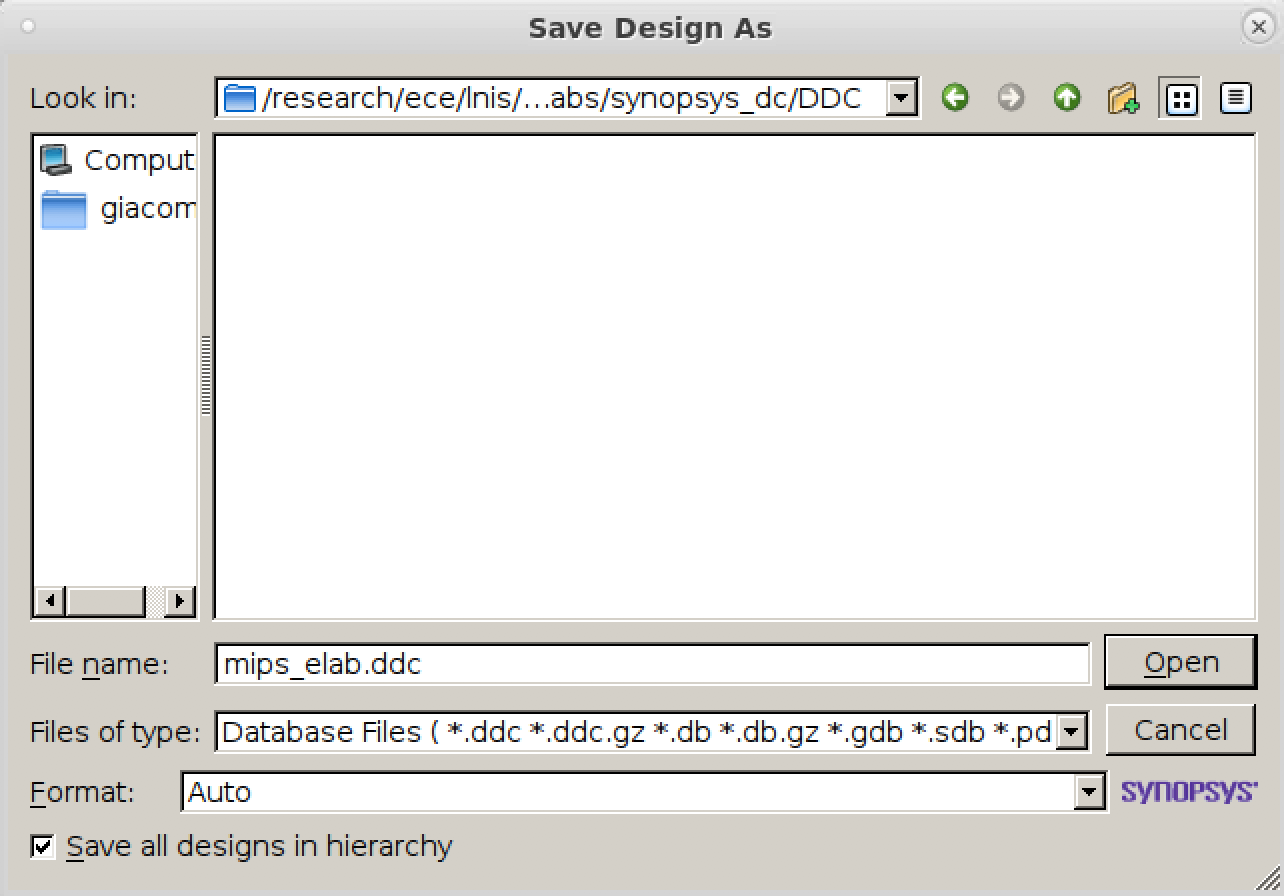
\includegraphics[scale=0.34]{figures/lab3_design_compiler/save_elab}
\caption{Saving the elaborated design}
\label{fig_save_elab}
	\end{wrapfigure}
At this step, it is recommended to save the elaborated design. To do so: 
\begin{enumerate}
	\item \textit {File -> Save As...}
	\item Save the design in the \textit{DDC} folder, as shown in Fig \ref{fig_save_elab} with the name: \textit{mips$\_$elab}.
	\item Select the DDC format. This is a binary format for storing the designs.
	\item Check the box {Save all designs in hierarchy.}
	\item Click on OK.
\end{enumerate}
}

\clearpage
Equivalent DC command:
	\begin{codeline}
	write -hierarchy -format ddc -output DDC/mips$\_$elab.ddc
\end{codeline}


When starting Synopsys DC again, it will be possible to directly load the elaborated design (if you want to change the constraints for instance or work on your project later) without re doing the previous steps by doing: \textit {File -> Read...} and selecting the appropriate design file in the \textit{DDC} folder.\\

Equivalent DC command: 
	\begin{codeline}
read$\_$ddc DDC/mips$\_$elab.ddc \newline
or \newline
read$\_$file -format ddc DDC/mips$\_$elab.ddc
\end{codeline}

\subsection{Linking the Design}
%\textbf{This part has te be rework after we get the IP from IMEC}

After elaborating the design, you may have noticed some warnings that means that for some components, no Verilog design entity has been defined:
\begin{figure}[!h]
	\centering
	
\includegraphics[scale=0.46]{figures/lab3_design_compiler/references}
	\caption{Unsolved references}
	\label{fig_references}
\end{figure}

The link operation defines the link libraries (the libraries that define the area/timing/power characteristics of other \textit{Intellectual Property} (IP) components, such as memories, analog blocks, \textit{etc.}). To do so: 
\begin{enumerate}
	\item \textit {File -> Link Design...}
	\item For your convenience, the linking libraries are already loaded.
	\item Click on OK.
\end{enumerate}
Equivalent DC command:
	\begin{codeline}
	link
\end{codeline}


\subsection{Specifying the Design Constraints}
During synthesis, constraints are typically timing and area. The design here is synchronous so a constraint has to be defined on the clock. The area constraint will ensure to get the smallest area possible. Synopsys DC will always consider the timing constraint in first and then will try to meet the area constraints if there are any. \\
To define the clock:
 \begin{enumerate}
 	\item Select the \textit{mips} instance in the hierarchy view (step 1 in Fig. \ref{fig_clock}) and open its schematic view with the Create schematic icon (step 2). This will open a new tab with the symbol view of the component.
 	\item Select the \textit{clk} pin. It should be on the left side, at the top (step 3).
	\item Go to: \textit {Attribute -> Specify Clock...} (step 4)
	\item Define a clock period of 30ns, as shown in Fig \ref{fig_clock} and a pulse width of 15ns (the unit is defined in the \textit{.db} file of your standard library. In our case, the unit is \textit{ns}). The clock waveform should be displayed if the clock specification is correct. The selected \textit{clk} pin is used as the port name.
	\item Click on OK (step 5).
\begin{figure}[!h]
	\centering
	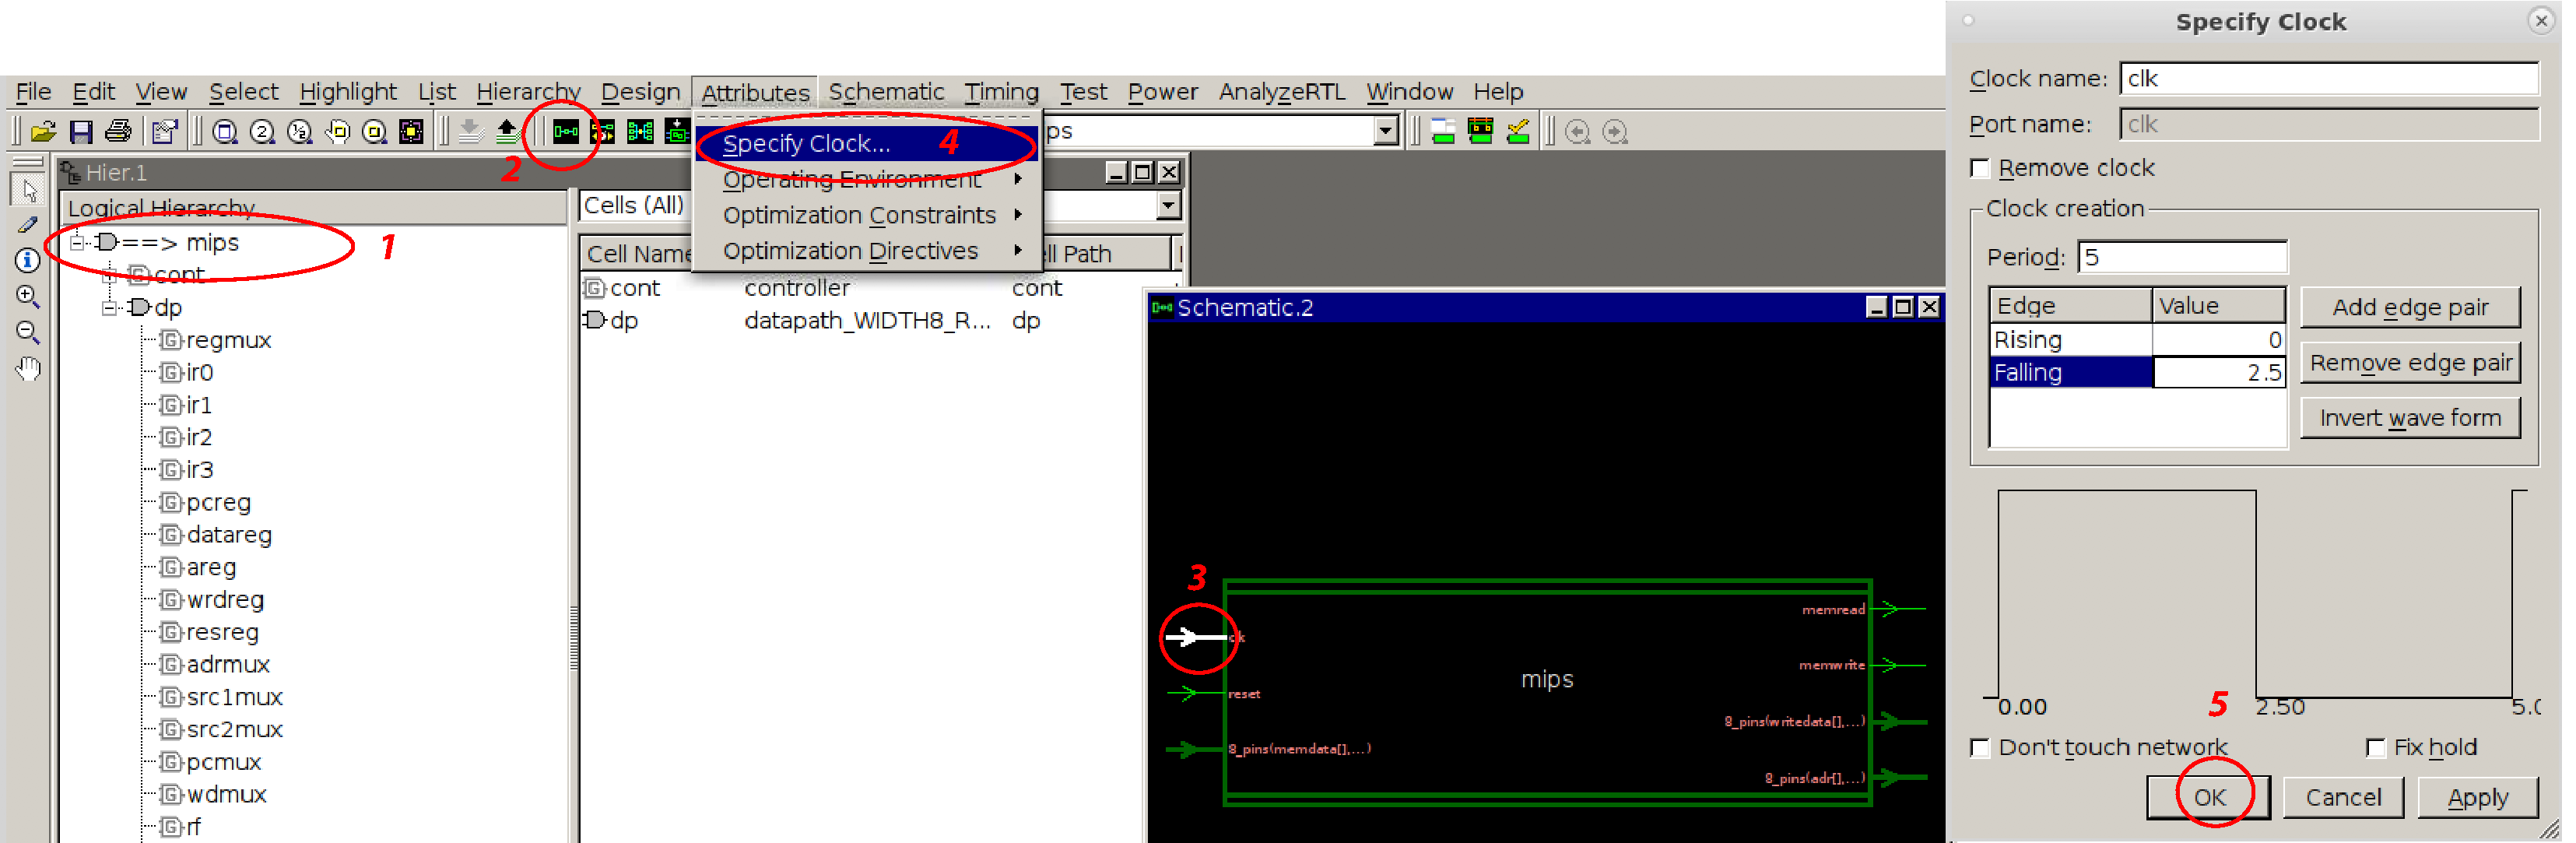
\includegraphics[scale=0.3]{figures/lab3_design_compiler/clockgene}
	\caption{Clock generation}
	\label{fig_clock}
\end{figure}


\end{enumerate}

\clearpage
Equivalent DC command:
	\begin{codeline}
create$\_$clock -name "clk" -period 30 -waveform $\{$ 0 15 $\}$ $\{$ clk $\}$
\end{codeline}

	\parbox[t]{\dimexpr\textwidth-\leftmargin}{%
	\begin{wrapfigure}[11]{r}{0.3\textwidth}
		\vspace{0mm}
		\centering
		\vspace{-\baselineskip}
		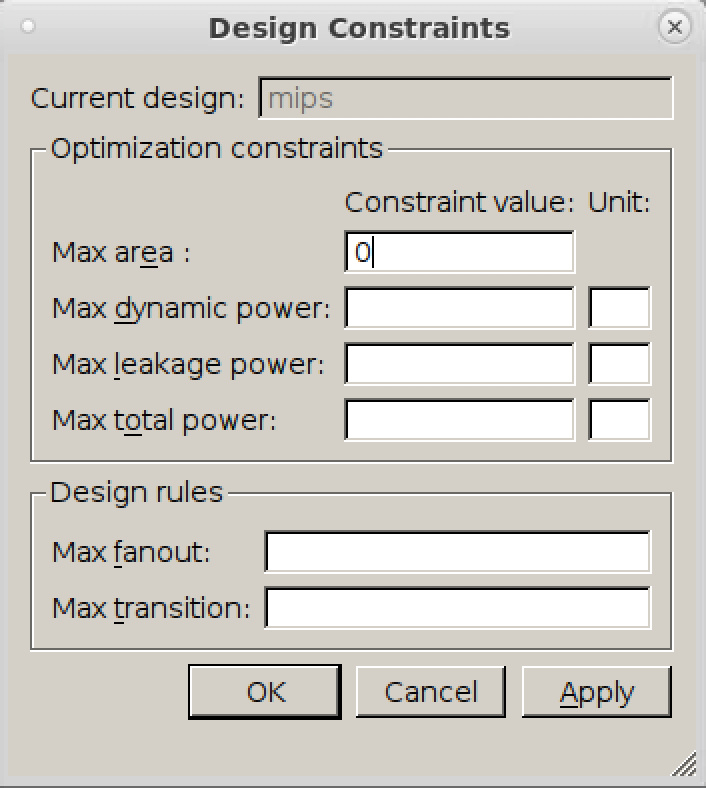
\includegraphics[scale=0.37]{figures/lab3_design_compiler/area}
\caption{Defining area constraint}
\label{fig_area}
	\end{wrapfigure}
To define the area constraint:
\begin{enumerate}
	\item \textit{Attributes -> Optimization Constraints -> Design Constraints...}
	\item Specify a Max area of 0 as depicted in Fig \ref{fig_area}. This is not realistic but this will tell DC to minimize the area without too much computation effort.
	\item Click on OK.
\end{enumerate}
Equivalent DC command: 
\begin{codeline}
	set$\_$max$\_$area 0
\end{codeline}
}

\subsection{Mapping the Design}
This phase (also called compilation phase) is technology dependent. It will assign the logic gates from the standard logic cell library defined in the .db file from the foundry to the generic gates obtained after the elaborated design by meeting the timing and area constraints.\\

	\parbox[t]{\dimexpr\textwidth-\leftmargin}{%
	\begin{wrapfigure}[11]{r}{0.42\textwidth}
		\vspace{0mm}
		\centering
		\vspace{-\baselineskip}
		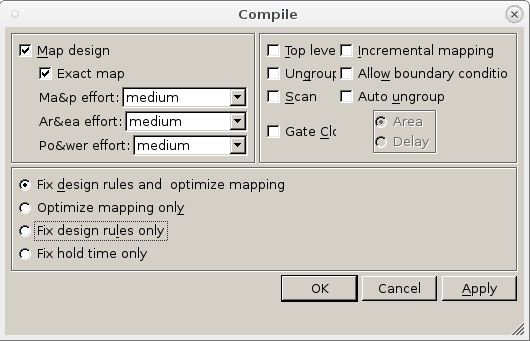
\includegraphics[scale=0.42]{figures/lab3_design_compiler/compile}
\caption{Compiling the design}
\label{fig_compile}
	\end{wrapfigure}
To map the design:
\begin{enumerate}
	\item \textit{Design -> Compile Design...}
	\item Do not change the default settings. The map effort is the amount of CPU time dedicated to select the proper gate from the cell library. A high effort will take more time. The area effort is the amount of CPU time spent during the area recovery phase (when DC try to meet the area constraint without breaking the timing constraint).
	\item Click on OK.
\end{enumerate}
}

Equivalent DC command:
	\begin{codeline}
compile -exact$\_$map -map$\_$effort medium -area$\_$effort medium
\end{codeline}

Once this phase is done, save the mapped design in the \textit{DDC} folder with the name: \textit{mips$\_$mapped}.

Equivalent DC command:
	\begin{codeline}
write -hierarchy -format ddc -output DDC/mips$\_$mapped.ddc
\end{codeline}


\begin{remark}
	As you did previously for the \textit{andblock} of the \textit{alunit}, you can display its schematic. This time, it will use the standard cells from the Skywater 130 \emph{nm} library and not the generic combinational logic functions (GTECH$\_$XXX elements) since your design is now mapped.
	\end{remark}

\subsection{Generating the Reports}

Once the mapping is done, many kind of reports can be generated. The DC command \textit{help report*} can give you a list of all the available report commands. Now, we are going to consider only some useful reports.

\subsubsection{Reporting all Violated Constraints}
This step will report if you design meets the timing and area constraints you specified. To do so:
 \begin{enumerate}
	\parbox[t]{\dimexpr\textwidth-\leftmargin}{%
	\begin{wrapfigure}[20]{r}{0.45\textwidth}
		\vspace{0mm}
		\centering
		\vspace{-\baselineskip}
	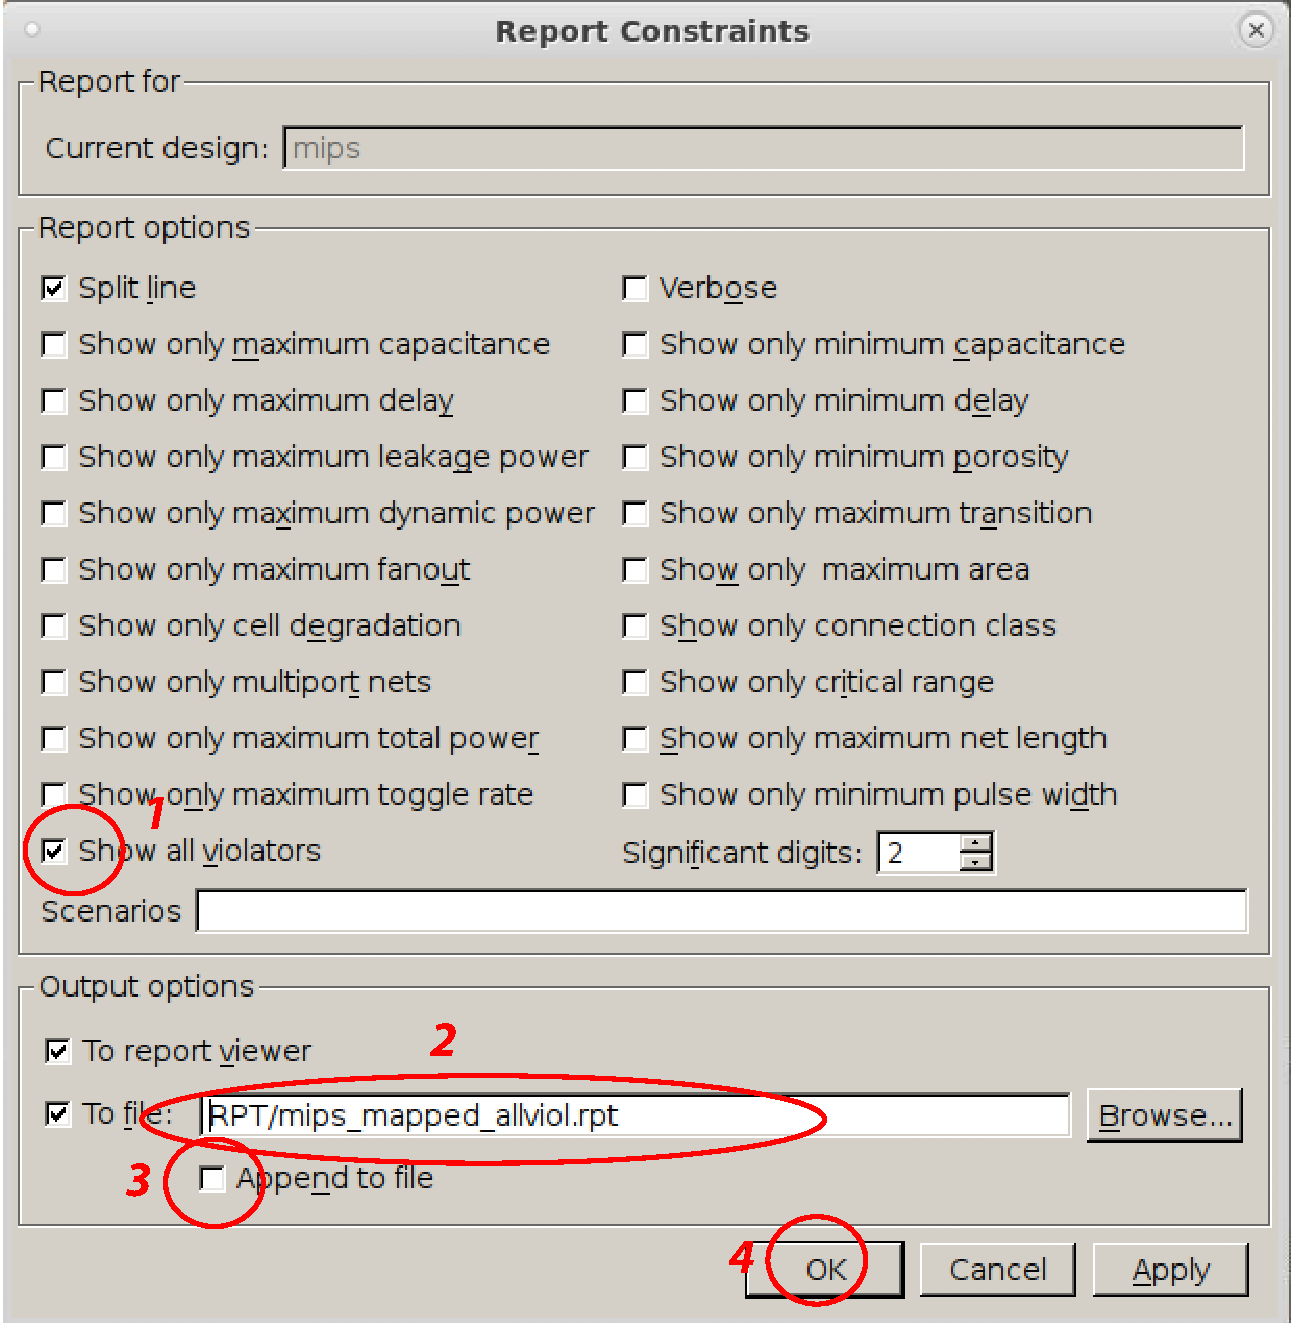
\includegraphics[scale=0.3]{figures/lab3_design_compiler/allviol}
\caption{Reporting all violated constraint}
\label{fig_allviol}
	\end{wrapfigure}
	\item Go to: \textit {Design -> Report Constraints...}
	\item As in Fig. \ref{fig_allviol}, check \textit{Show all violators} and \textit{To report viewer} (that means to the console). Uncheck \textit{Append to file}. In that way, if the file was already existing, it would overwritten its content.
	\item Check \textit{To file} and specify the path: \textit{RPT/mips$\_$mapped$\_$allviol.rpt}
	\item Click on OK.
	\item On the console terminal, you should only see an area constraint violation. This is normal since the area has been set (artificially) to 0 and the clock period constraint is large.
}
\end{enumerate} 

Equivalent DC command:
	\begin{codeline}
report$\_$constraint -nosplit -all$\_$violators > RPT/mips$\_$mapped$\_$allviol.rpt
\end{codeline}



%\subsubsection{Reporting the Design Hierarchy}
%\begin{enumerate}
%	\item Go to: \textit {Design -> Report Design Hierarchy...}
%	\item Select the parameters as in Fig. \ref{fig_hierarchy}.
%	\item Check \textit{To file} and specify the path: \textit{RPT/misc$\_$top$\_$mapped$\_$hierarchy.rpt}
%	\item Click on OK.
%\end{enumerate} 
%\begin{figure}[!h]
%	\centering
%	\includegraphics[scale=0.6]{figures/hierarchy}
%	\caption{Reporting the design hierarchy}
%	\label{fig_hierarchy}
%\end{figure}

%Equivalent DC command: \codev{./files/hierarchy.c}


%The log window now displays the mapped hierarchy of your design. All standard cells are now taken from the standar cell library.
\subsubsection{Reporting the Area}


 \begin{enumerate}
	\parbox[t]{\dimexpr\textwidth-\leftmargin}{%
		\begin{wrapfigure}[22]{r}{0.45\textwidth}
			\vspace{0mm}
			\centering
			\vspace{-\baselineskip}
	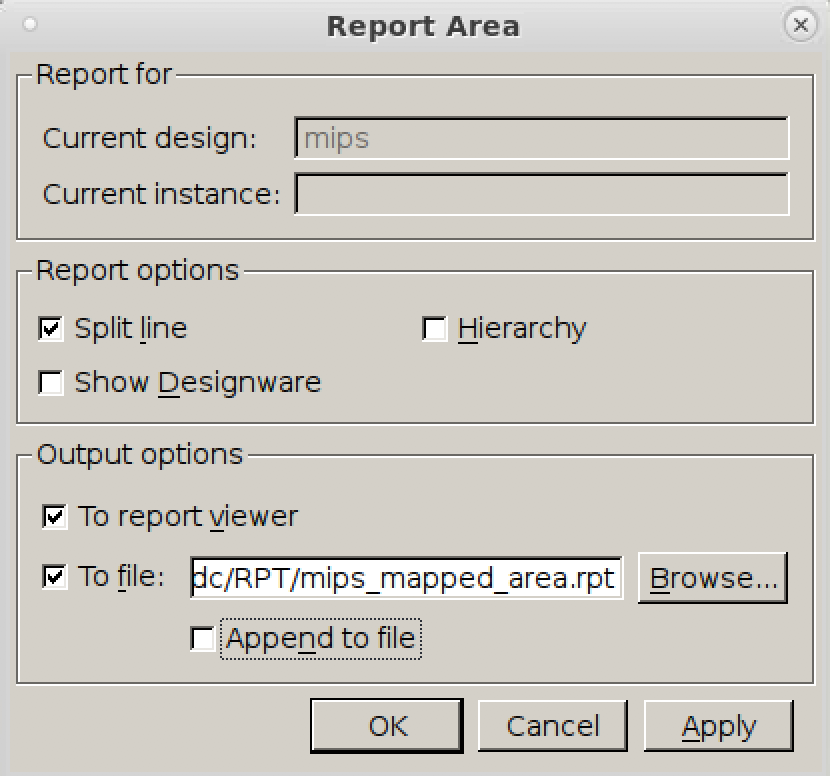
\includegraphics[scale=0.4]{figures/lab3_design_compiler/reportarea}
\caption{Reporting the design area}
\label{fig_reportarea}
		\end{wrapfigure}
	\item Go to: \textit {Design -> Report Area...}
\item Select the parameters as in Fig. \ref{fig_reportarea}.
\item Check \textit{To file} and specify the path: \textit{RPT/mips$\_$mapped$\_$area.rpt}
\item Click on OK. \newline \newline
Equivalent DC command:

\begin{codeline}
	report$\_$area -hierarchy -designware > RPT/mips$\_$mapped$\_$area.rpt
\end{codeline}
In the log view, you can now see the area report with the total area, the combinational area, the noncombinational area (registers and RAM) \textit{etc}. The area is generally provided in square microns (depending on the cell library). The net interconnect area is, for this particular cell library, not defined as the supplied wire load
models from the timing library does not provide any area values. This is why the total area is said to be undefined so for this step, consider the total cell area as your design area. The actual net area will be known after the back-end flow in the next lab.
	}
\end{enumerate} 
\clearpage


\subsubsection{Reporting the Timings}

This report will give an important timing: the critical path. This is the path in your design which takes the longest time to be propagated.
 \begin{enumerate}
	\parbox[t]{\dimexpr\textwidth-\leftmargin}{%
		\begin{wrapfigure}[22]{r}{0.45\textwidth}
			\vspace{0mm}
			\centering
			\vspace{-\baselineskip}
	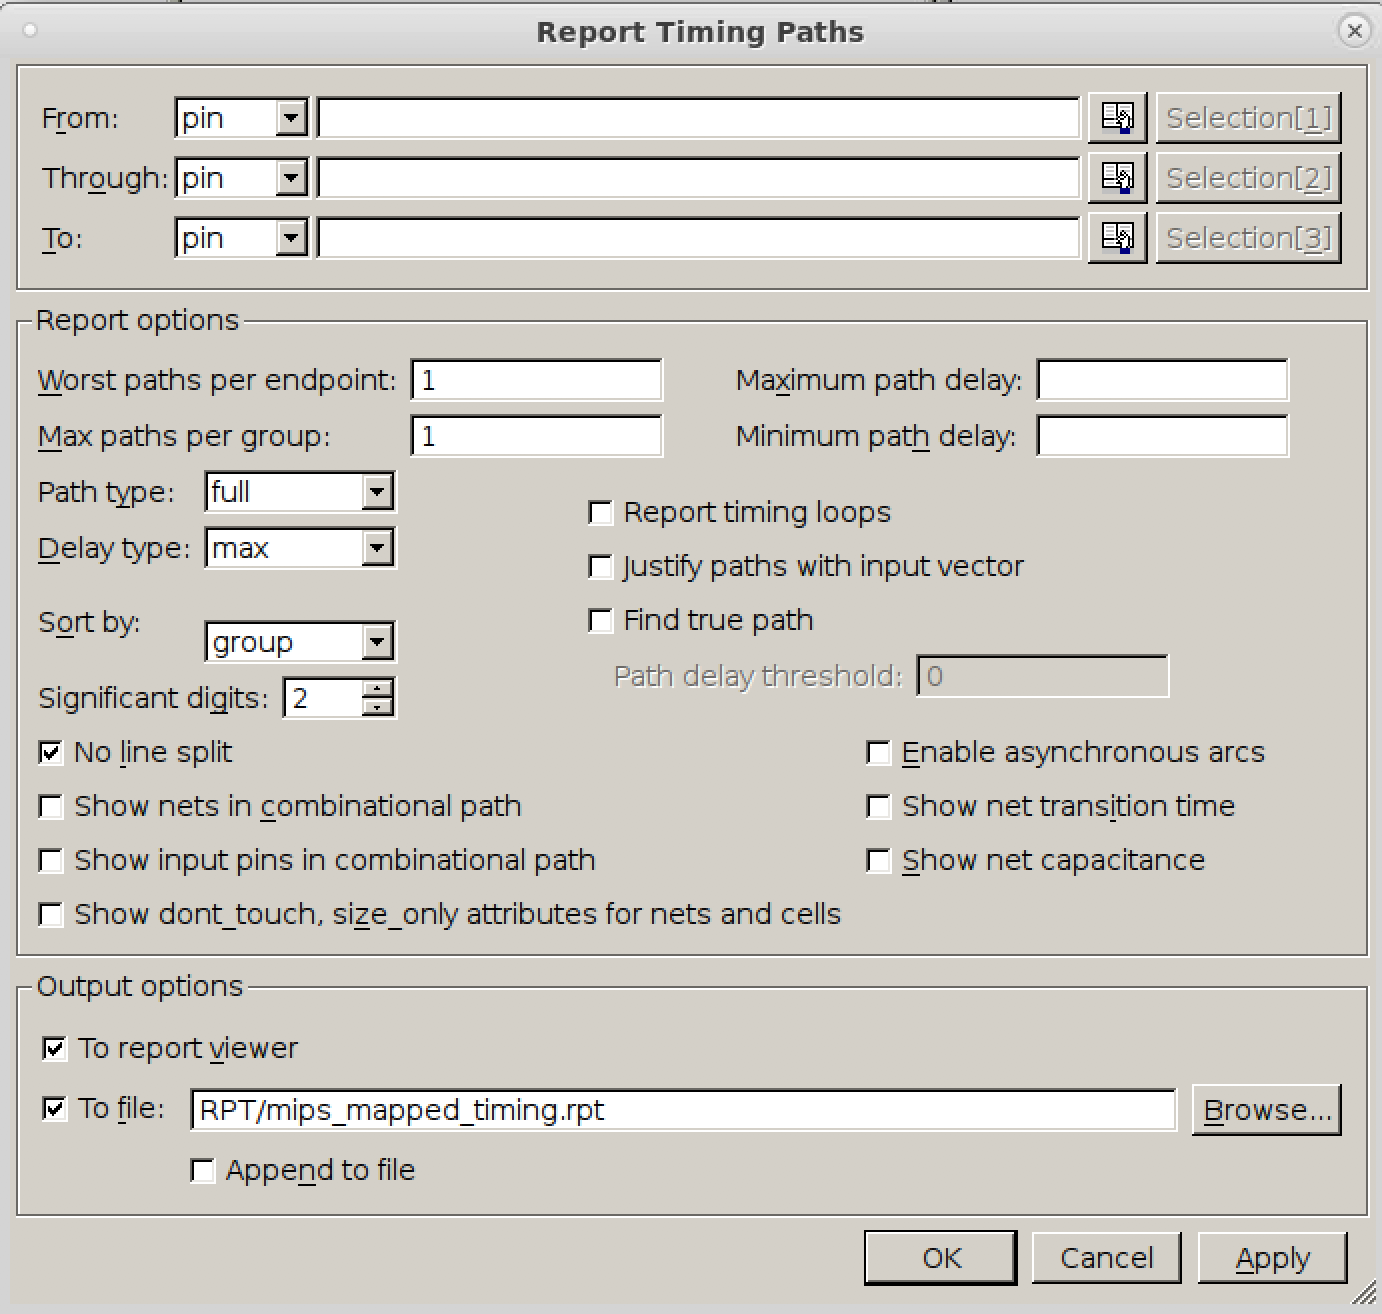
\includegraphics[scale=0.32]{figures/lab3_design_compiler/reportiming}
\caption{Reporting the critical path}
\label{fig_reportiming}
		\end{wrapfigure}
	\item Go to: \textit {Timing -> Report Timing Path...}
\item Select the parameters as in Fig. \ref{fig_reportiming}.
\item Check \textit{To file} and specify the path: \textit{RPT/mips$\_$mapped$\_$timing.rpt}
\item Click on OK. \\ \\
Equivalent DC command:
\begin{codeline}
	report$\_$timing > RPT/mips$\_$mapped$\_$timing.rpt
\end{codeline}
A new window should open where you can see the slack of your mapped circuit. The slack is the difference between the required time and the longest arrival time (which is the critical path of your circuit). A negative slack value indicates a timing violation and a positive slack indicates that your design meets the timing constraints.
	}
\end{enumerate}



\begin{remark}
The timing analysis only consider approximate values for the interconnection delays. Accurate values will be only known after the place and route step (in the next lab). 
\end{remark}

\subsubsection{Reporting the Power}
This report will give the power consumption of your circuit, which is an important parameter in VLSI design.

 \begin{enumerate}
	\parbox[t]{\dimexpr\textwidth-\leftmargin}{%
		\begin{wrapfigure}[26]{r}{0.5\textwidth}
			\vspace{0mm}
			\centering
			\vspace{-\baselineskip}
	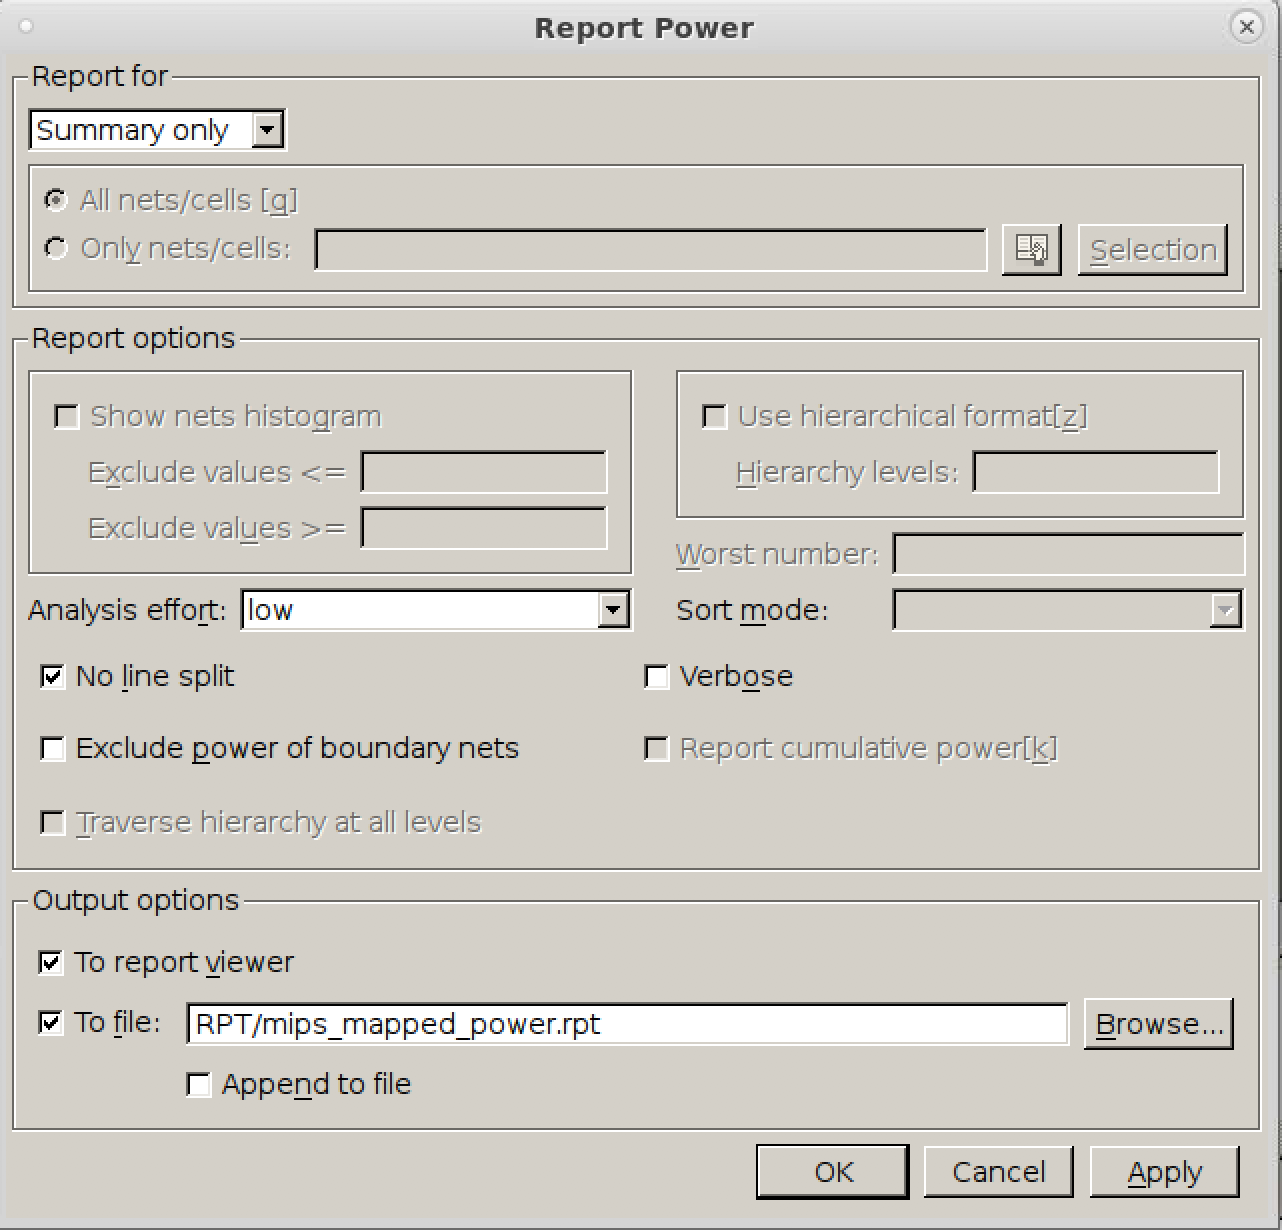
\includegraphics[scale=0.3]{figures/lab3_design_compiler/reportpower}
\caption{Reporting the power}
\label{fig_reportpower}
		\end{wrapfigure}
	\item Go to: \textit {Design -> Report Power...}
\item Select the parameters as in Fig. \ref{fig_reportpower}.
\item Check \textit{To file} and specify the path: \textit{RPT/mips$\_$mapped$\_$power.rpt}
\item Click on OK. \\ \\
Equivalent DC command:

\begin{codeline}
	report$\_$power -nosplit -analysis$\_$effort low > RPT/mips$\_$mapped$\_$power.rpt
\end{codeline}

	}
\end{enumerate}

\clearpage

\subsection{Exporting the Synthesized Design}
This part will generate all the necessary files for the next step: Place $\&$ Route.

\subsubsection{Generating the Verilog Gate-Level Netlist}
This step will generate the verilog gate-level netlist, i.e, the netlist of your design which only contains standard cell from the targeted technology library and no more behavioral verilog.

\begin{enumerate}
	\item Go to: \textit {File -> Save As...}
	\item Select the parameters as in Fig. \ref{fig_save_verilog}. Don't forget to select the appropriate format and the appropriate path.
	\item Click on OK.
\end{enumerate} 

\begin{figure}[!h]
	\centering
	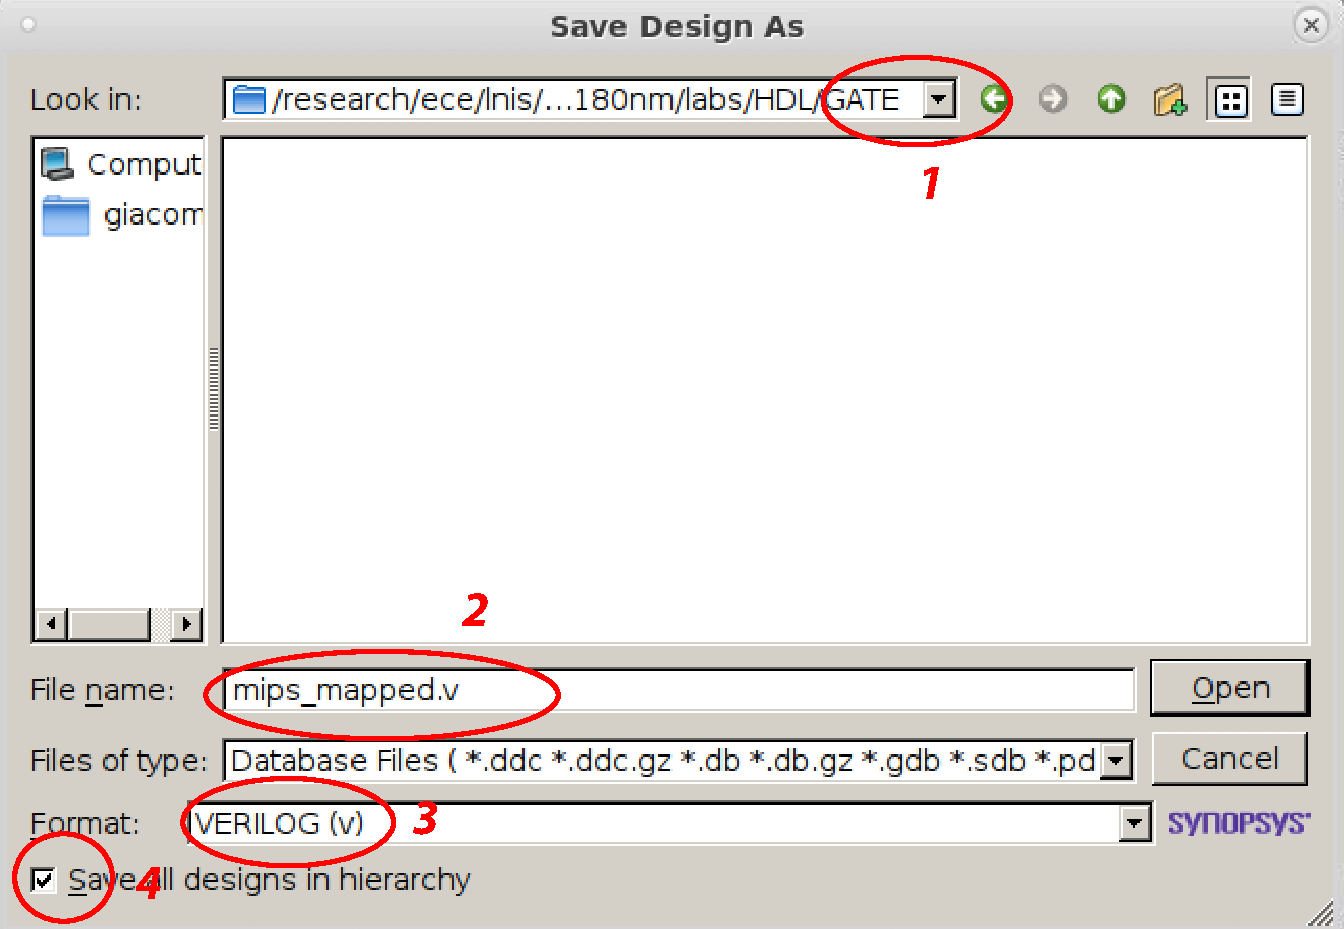
\includegraphics[scale=0.5]{figures/lab3_design_compiler/save_verilog}
	\caption{Exporting the verilog gate-level netlist}
	\label{fig_save_verilog}
\end{figure}
Equivalent DC command: 

\begin{codeline}
write -format verilog -hierarchy -output ../HDL/GATE/mips$\_$mapped.v
\end{codeline}

\subsubsection{Generating the SDF timing file}
This step will generate the \textit{Standard Delay Format} (SDF) file which includes the gate delays. It is then used for post-synthesis functional verification (with Modelsim\textsuperscript{\tiny\textregistered} for instance). To do so, you need to use the console terminal:

Equivalent DC command:
\begin{codeline}
write$\_$sdf -version 2.1 SDF/mips$\_$mapped.sdf
\end{codeline}

\subsubsection{Generating the Constraint File}
This step will generate the constraints file which specifies the design constraints. The \textit{sdc} format can latter be read by the Place $\&$ Route tools (like synopsys PrimeTime\textsuperscript{\tiny\textregistered} or Cadence Innovus\textsuperscript{\tiny\textregistered}). 

Equivalent DC command: 
\begin{codeline}
	write$\_$sdc -nosplit SDC/mips$\_$mapped.sdc
\end{codeline}


\subsubsection{Using a Tcl Script}
When designs are more complex or if you want to repeat the previous tasks, it is recommended to use scripts and to run those from the Synopsys DC command line. Synopsys Design Compiler supports the Tcl language for building scripts. All the commands specified in this manuscript can be grouped into a single Tcl script file which is in your folder: \textit{synthesis.tcl}. You can now perform the same steps as before by modifying the clock constraint (and use the script to go faster). To do so:
\begin{enumerate}
	\item Open the \textit{synthesis.tcl} file in your \textit{design$\_$compiler/SCRIPTS} folder and try to find the line where the clock is specified and modify its value and save the script.
	\item In the Synopsys DC terminal, run: 
	\begin{codeline}
		source SCRIPTS/synthesis.tcl
	\end{codeline}

\end{enumerate} 



	\begin{exercise}\
	\vspace{-6mm}
	\begin{enumerate}
\item Optimize your design specifying a tighter clock constraint (do not forget that your timing slack has to remain positive or equals to 0). To do so, you need modify the \textit{source synthesis.tcl} and run it.
\item Provide the screenshots of the critical path, the area and the power report of your final optimized design. Also report the number of combinational and sequential cells.
\item Report the smallest clock period you achieved while keeping a positive slack.
	\end{enumerate}
	\vspace{-5mm}
\end{exercise}


\begin{checkpoint}\label{check1}
	Please call an assistant and show him that you generated the \textit{.sdc} file and the verilog gate-level netlist file correctly.
\end{checkpoint}

\section{Assignment and Checkpoint Summary}
Write a report and answer the assignment. Do not forget to validate the checkpoint by an assistant before the end of the lab.